%(i) The extent to which the proposed project methodology is meritorious, including consideration of the extent to which: (A) The proposed project shows awareness of the state-of-the-art for current, related products. (B) The proposed project employs appropriate concepts, components, or systems to develop the new or improved product. (C) The proposed project employs appropriate samples in tests, trials, and other development activities. (D) The proposed project conducts development activities in appropriate environment(s). (E) Input from individuals with disabilities and other key stakeholders is obtained to establish and guide proposed development activities. (F) The applicant identifies and justifies the stage(s) of development for the proposed project; and activities associated with each stage. 

\subsubsection{Background and State-of-the-Art}

\textbf{Non visual Navigational Aids}

Tool development for low vision and blind populations has ranged from audible navigational aids, to smart canes and wearable technologies that can communicate with instrumented environments providing enhanced information to pedestrians as they travel. 

In contrast, maps have potentially richer content. Indeed, maps are an important tool for  navigation because they help people to understand the spatial layout of the targeted environment. However, most maps are inherently visual. One solution that has a long history in the Blind and Blind-deaf community is tactile maps. Common approaches include embossing, printing ind Braille, and "swell" (microcapsule) paper. These approaches can be used to create a two-layer tactile visualization from an image (\textit{e.g.}, \cite{miele2006talking}). However such machines can be very costly \cite{rice2005design}, are not readily available, and lack the expressive range of a solution that can vary more in height. While vacuum-forming has more height, it depends on a pre-existing form, which limits its customizability. Finally, the design of a tactile map requires expertise to be easily understandable \cite{tatham1991design}.


\textbf{Tactile Maps}

The utility of tactile maps in wayfinding and orientation for people with visual impairments is well established. Tactile maps provide users with information that facilitates enhanced orientation and navigation (Erin 2009; Espinosa et al. 1998), while also giving form to the pedestrian environments that impact the way everyone moves through space. 
Tactile maps have been demonstrated to contribute to people’s ability to learn new routes, and are an important source of geographical information, particularly when people are learning new environments (Blades, Ungar, and Spencer 1999). 

As with graphic maps, there a variety of ways in which tactile maps can be used.  When compared to a group that received a verbal description, blind and low vision pedestrians were shown to gain significantly more spatial knowledge by experiencing a new urban environment with a tactile map (Espinosa et al. 1998).   Tactile maps provide an opportunity for users to orient in urban and rural environments (Rowell and Ungar 2003c), as well as in more confined spaces such as buildings, conference centers or campuses (Erin 2009).  These physical representations of the environment can be used while actively navigating or orienting, but also facilitate learning a route prior to embarking on a journey (Espinosa et al. 1998).  Due to a lack of experience with tactile maps not all people that are blind or have low vision feel comfortable using this type of navigational aid (Erin 2009).  However, tactile graphics are generally accepted as useful for providing contextual information that is not directly related to mobility, such as city’s location within a state (Erin 2009).

\textbf{Fabricated Tactile Maps}

As noted earlier, traditional production methods can be very costly \cite{rice2005design}, difficult to reproduce, non-scalable, and the technology for creating these artifacts are not readily available. 3D printing, also called consumer-grade manufacturing, is ideally suited for bringing  down costs when customization is needed. 3D printers are now available for a price point  as low as 200 dollars, and services that 3D print any valid file are also widely available. Thus,  3D printing is democratizing access to manufacturing of tangible, physical objects. 


Despite  indications that improving mass fabrication techniques for the production of tactile maps 
could be beneficial for people with both visual and hearing loss, this area remains relatively unexplored in contrast to the body of work on mobile navigation apps and other connected devices that serve as navigational aids. Recent work has begun to explore the use of 3D 
printing to reduce cost. 
For example, it is now possible to requisition a custom, laser-cut topographical map on ETSY \cite{etsy} or purchase custom 3D printed topographic models through companies such as Sightline \url{sightlinemaps.com} or PrintMyRoute \url{www.printmyroute.xyz}. 

The accessibility community has added its own spin to these technologies. For example TouchMapper \textit{touch-mapper.org} is a free service that will create a tactile map using embossing or 3D printing and help connect you to existing online printing services or print it yourself.  This service focuses on showing streets, and can be customized for size, inclusion of buildings and some other features. However it too does not include route finding or landmark identification. There are additional issues with the approach since the maps do not designate topography, do not represent pedestrian-centric information (such as what type of pedestrian signal is at a crossing), nor other important environmental representations that would allow a traveler who is blind or Deaf-blind make informed decisions about choosing a route. 
Specifically, the services do not include features intended to support Deaf-blind users, and do not support travel activities such as route finding and landmark identification as a result. Other than our preliminary participant study, we are not aware that these systems have been tested with Deaf-blind individuals.


To summarize, tactile maps are not new to the cartographic record. Their value in facilitating orientation and navigation for the low vision and blind communities has been well established. However, their scope and availability has been greatly limited in the past by high production costs and limited interest from fields traditionally invested in map making and design.  3D printing has significantly reduced the costs of producing such maps, but to our knowledge no existing product has enhanced 3D printed maps with optimization and customization, making our product an important addition to this space. 


\subsubsection{Previous Development}

Our previous development focused on finding usable abstractions in the map to increase map content and user understanding of the pedestrian environment \ac{cite ASLA 2017}.
It is important to note that in our pilot work (Section \ref{sec:pilot}) users found the pedestrian environment more legible when the 3D printed maps did not directly model 1:1 the environments they represented. The greatest success with users (as measured by their later explanation of their mental model of the area) was perceived with maps that abstracted some features and omitted others in order to emphasize the information deemed important in the pedestrian environment. More space for the pedestrian information of interest was created through the reduction of building footprints by 70\% , and indenting the  them from the base rather than extruding. This still allowed users to understand the global form of the landscape, identify the buildings, and still incorporate rich information about sidewalks and intersections.


\subsubsection{Proposed Development}

We have a pipeline to create fabricated tactile maps that currently requires manual interventions. The work task for this development activity is to completely automate this workflow, as shown on the right side of Figure \ref{fig:TactileMapTileDev}.

\ac{explain the development activity of making the pipeline automated in words}

\begin{figure}
    \centering
    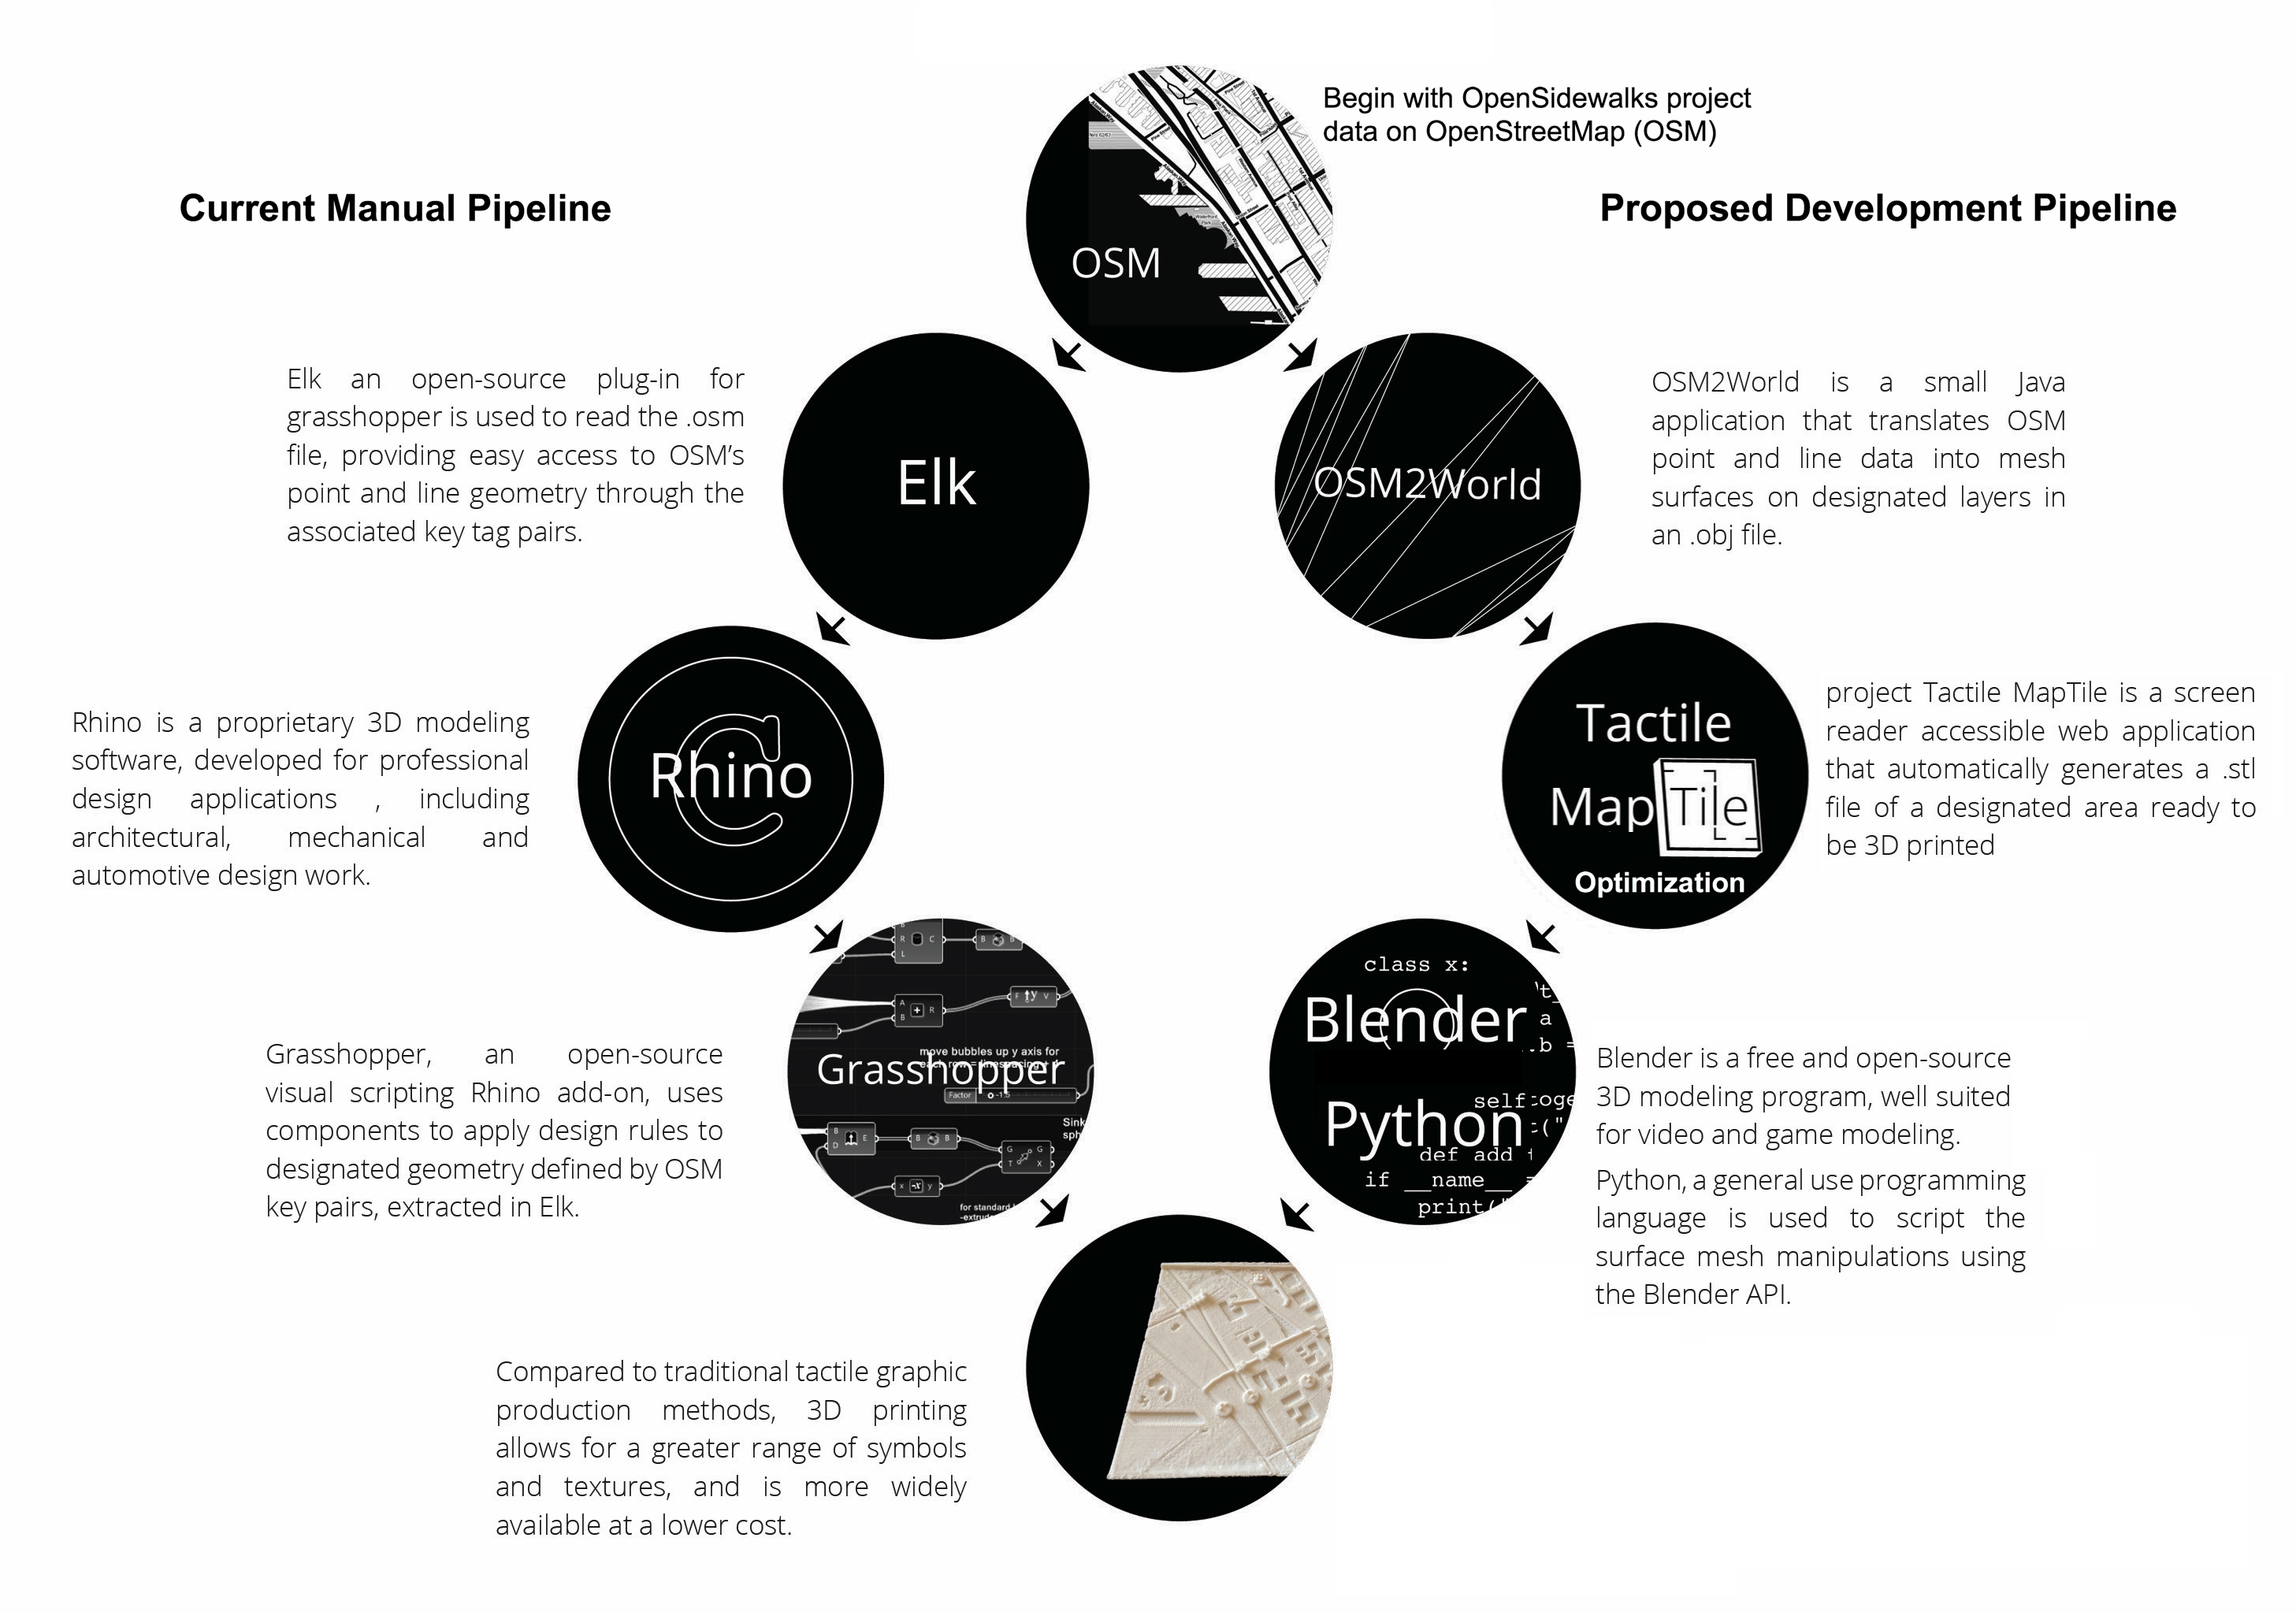
\includegraphics[width=5.5in]{pics/TactileMaptilePipeline.jpg}
    \caption{Tactile Map Tile Development Pipeline}
    \label{fig:TactileMapTileDev}
\end{figure}


\begin{comment}

\ac{ THIS SECTION IS A HODGE PODGE. NEED TO DESCRIBE: WHAT WILL BE DEVELOPED, TECHNICAL EVAL (SUCCESS METRIC) AND USABILITY EVAL (METRICS)


While tactile interactions have been studied extensively by others (\textit{e.g.}, see this review \cite{o2015designing}) as well as our team (\ac{cite ASLA 2017}), the specific design considerations for tactile maps are not as well understood, particularly for Deaf-blind individuals. In addition, no computational model that takes these variables into account exists (this is the subject of Section\ref{sec:optimize}).

to do: Megan to describe how she will create atomic semantic features to be included in the models. Also need to describe how she will test that the material composition is comfortable for the users, and how she will engage participatory design methods in figuring out the right scale, the right Braille, legend, etc., basically need to respond to the enumerated point considerations
%(C) The proposed project employs appropriate samples in tests, trials, and other development activities. (D) The proposed project conducts development activities in appropriate environment(s). (E) Input from individuals with disabilities and other key stakeholders is obtained to establish and guide proposed development activities. (F) The applicant identifies and justifies the stage(s) of development for the proposed project; and activities associated with each stage. }
\end{comment}

\subsubsection{Validation}

The following validation statements should be tested and hold true if the design goal for this development activity is met: 

The developed pipeline improves reproducibility and accessibility of map information options relative to prevailing options for travelers who are Deaf-blind.

The developed pipeline does not exceed in cost or time over prevailing services.

Here we describe our validation tests for both statements. The data elements and sources are referencing tests and data collection that will occur with our community partners. These data collection activities are described in later sections with greater detail.

\textbf{Validation Statement 1:
The developed pipeline improves reproducibility and accessibility of map information options relative to prevailing options for travelers who are Deaf-blind.}

\texttt{Performance Metrics:} Change in perception of information content and accessibility of information during a two-phased alpha and beta approach, demonstrating improvements in mental models of area, satisfaction and feedback. Also used as metrics would be survey questions designed to assess the baseline access to map information nationally via the national outreach survey instrument (described in Section \ref{test:baseline}). Additionally, responses to questions regarding the perception of accessibility and reproducibility of mapping options for individuals who are Deaf-blind will be used.

\texttt{Data Elements \& Sources:}
Early Development Baseline Survey (Section \ref{test:baseline}) and 
Surveys of User Groups: alpha and beta populations (Section \ref{test:usersurvey}).

\texttt{Analysis Procedure:}
The survey data collectively would be used to evaluate this hypothesis.  The survey responses will be aggregated according to specific metrics that capture relevant information, such as the percentage of users who feel as though the Tactile Map Tile option has (1) increased their overall access to map information, or (2) increased access to better information.  
The survey will be deployed to the identified beta user group. Since the survey will include the elderly along with younger adults — all of which will be identifiable through survey questions — we will disaggregate the analysis on separate demographic cohorts as necessary.

\textbf{Validation Statement 2:
The developed pipeline does not exceed in cost or time over prevailing services.}

\texttt{Performance Metrics:} Change in cost and time to access tactile map services with our alpha and beta populations. Also used as metrics would be survey questions designed to assess the baseline cost and time to access tactile and other map information nationally via the national outreach survey instrument (described in Section \ref{test:baseline}). 

\texttt{Data Elements \& Sources:}
Early Development Baseline Survey (Section \ref{test:baseline}) and 
User Groups: alpha and beta populations (Section \ref{test:usersurvey}). Please see test description for suggested population sample.

\texttt{Analysis Procedure:}
The survey data collectively would be used to evaluate this hypothesis.  The survey responses will be aggregated according to specific metrics that capture relevant information. No disaggregation by demographics will be used for this validation.

\begin{comment}

\textbf{usability evaluation for map scale and symbol size}
Due to 3D print bed constraints, map tiles were limited to ~8” x 5.5”. At this scale, 3 tiles are needed in order to capture an area that includes approximately 1.5 squared mile. Based on preliminary feedback from expert users, basic features of the urban pedestrian environment were legible at this scale.  Further usability testing and symbol development will be conducted during our development project in order to assert that this scale is appropriate for use as a navigational aid. In our pilot \ref{sec:pilot} case study map series was printed with slight variation in symbol style, and size on each tile for user testing. In our development project participatory process, we will increase the variations produced and exaggerate some of the detailed features to assess user preferences for map scale and symbol size under different contexts of map use.


From a research perspective, one open problem is combining tactile maps and smartphones. By embedding capacitive touch sensing capabilities in tactile maps, it is possible to provide audio feedback about the region someone is touching \cite{taylor2016customizable, rusu2010semantic,gotzelmann2016lucentmaps}. 

Finally, questions remain about the ability of tactile maps to support route finding (as opposed to orientation). For example, Gual \textit{et al.} found that standard 3D printed maps can improve memorization in route finding, but could not be used autonomously without collaborator support \cite{gual2012visual}. However, they did not explore a wide range of tactile variables to support interpretation. 


\end{comment}

